% Created 2021-08-29 Sun 09:23
% Intended LaTeX compiler: pdflatex
\documentclass[11pt,twoside,landscape]{article}
\usepackage[utf8]{inputenc}
\usepackage[T1]{fontenc}
\usepackage{graphicx}
\usepackage{grffile}
\usepackage{longtable}
\usepackage{wrapfig}
\usepackage{rotating}
\usepackage[normalem]{ulem}
\usepackage{amsmath}
\usepackage{textcomp}
\usepackage{amssymb}
\usepackage{capt-of}
\usepackage{hyperref}
\usepackage[top=2cm,bottom=2cm,right=2cm,left=2cm,landscape]{geometry}
\usepackage{multicol}
\usepackage{enumitem}
\setlist{noitemsep}
\setlength{\parindent}{0pt}
\setlength{\columnseprule}{0.2pt}
\setcounter{secnumdepth}{0}
\author{Olivier Lischer}
\date{\today}
\title{Automaten und Sprachen}
\hypersetup{
 pdfauthor={Olivier Lischer},
 pdftitle={Automaten und Sprachen},
 pdfkeywords={},
 pdfsubject={},
 pdfcreator={Emacs 27.2 (Org mode 9.4.6)}, 
 pdflang={English}}
\begin{document}

\maketitle
\setcounter{tocdepth}{2}
\tableofcontents

\begin{multicols}{3}
\section*{Week 1\hfill{}\textsc{empty}}
\label{sec:orgb12051f}
\subsection*{Basics}
\label{sec:orga08e0b3}
Das folgende ist \textbf{kein} Graph, weil jede Kante brauch einen Anfangs- und Endknoten.
\begin{center}
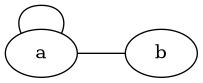
\includegraphics[width=.9\linewidth]{static/img/autospr/no_graph.png}
\end{center}

Dies ist allerdings ein Graph (Ein Anfangskonten und Endknoten definiert durch die Pfeile).
\begin{center}
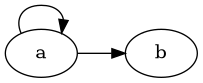
\includegraphics[width=.9\linewidth]{static/img/autospr/graph.png}
\end{center}

\subsection*{Sprache}
\label{sec:org413e269}
\begin{itemize}
\item Alphabet: normalerweise griechische Buchstaben (\(\Sigma\))
\item Die Menge aller Wörter: \(\Sigma^*\)
\item Das leere Wort: \(\epsilon\)
\item Die Sprache ist eine Teilmenge aller Wörter: \(L \subset \Sigma^*\)
\end{itemize}

\section*{Week 2}
\label{sec:org8f6b847}
\subsection*{DEA (Deterministische endliche Automaten)}
\label{sec:org3b4cb19}
\subsubsection*{Definition}
\label{sec:org5ec67fa}
\begin{enumerate}
\item \(Q\) endliche Menge von Zuständen
\item \(\Sigma\) endliche Menge, das Alphabet
\item \(\delta: Q \times \Sigma \to Q\) Übergangsfunktion
\item \(q_0 \in Q\) Startzustand
\item \(F \subset Q\) Menge der Akzeptiertzustände

Von jedem Zustand, muss es für jedes Zeichen genau einen Übergang geben. Es ist also zu jeder Zeit klar, wo der Automat genau ist.
\end{enumerate}
\subsubsection*{Beispiel}
\label{sec:orgc2f90df}
\begin{center}
\begin{tabular}{lrl}
q & a & \(\delta(q,a)\)\\
\hline
q0 & 0 & q0\\
q0 & 1 & q1\\
q1 & 0 & q0\\
q1 & 1 & q1\\
\end{tabular}
\end{center}

\begin{center}
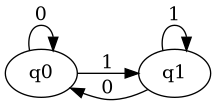
\includegraphics[width=.9\linewidth]{static/img/autospr/even_binary_dea.png}
\end{center}

\subsubsection*{Myhill-Nerode}
\label{sec:orge949d94}
\begin{quote}
Ist L eine requläre Sprache, dann wird L von dem endliche Automaten \(A = (Q,\Sigma,\delta,q_0,F)\) akzeptiert mit
\end{quote}
\begin{align*}
Q = \{L(w) | w \in \Sigma^*\} \\
q_0 = L \\
F = \{q \in Q | \epsilon \in q\} \\
\delta = Q \times \Sigma \to Q : (L(w),a) \mapsto L(wa) 
\end{align*}

Dieser Satz kann benutz werden, um zu entscheiden ob eine Sprache regulär ist: Wenn \(\{L(w) | w \in \Sigma^*\}\) endlich ist, ist die Sprache regulär. Als Beispiel ist die Sprache \(\{0^n1^n | n \in \mathbb{N}\}\) über \(\Sigma = \{0,1\}\) nicht regulär, da man unendliche viele Zustände benötigt. Eine DEA hat \textbf{kein} Gedächnis.
\subsubsection*{Minimaler Automat}
\label{sec:org5a5cabf}
Automaten können reduziert werden zu einem minimalen Automaten. Wenn zwei verschiedene DEAs auf den selben minimalen DEA reduziert werden können, akzeptieren die beiden Automaten die selbe Sprache. Der minimale Automat kann mit dem Kreuzchen Algorithmus konstruiert werden.
\section*{Week 3}
\label{sec:org8d6d0cf}
\begin{itemize}
\item Nicht deterministische endliche Automaten
\begin{itemize}
\item "Könnte"-Automat
\item Transformation NEA -> DEA
\end{itemize}

\item Mengenoperationen
\begin{itemize}
\item Vereinigung
\item Durchschnitt (Produktautomat)
\item Differenz
\end{itemize}
\end{itemize}

\subsection*{Pumping Lema - Reguläre Sprachen}
\label{sec:org0c9c8bc}
Mit dem Pumping Lema kann erkennt werden, ob eine Sprache nicht regulär ist. Wenn das Wort lange genug ist (Puming Length N), dann kann das Wort in drei Teile (x, y, z) aufgeteilt werden:
\begin{enumerate}
\item \(|y| > 0\)
\item \(|xy| \leq \mathbb{N}\)
\item \(xy^kz \in L  \forall \geq 0\)
\end{enumerate}

\subsubsection*{Beispiel}
\label{sec:org9fa450c}
Beweise dass \(L = \{0^n1^n | n \in \mathbb{N}\}\) nicht regulär ist.

\begin{enumerate}
\item Annahme \(L\) sei regulär
\item Da regulär und lange genug, gibt es eine Pumping Length N
\item Bilde ein Wort mit der Länge N (z.B. 0\textsuperscript{N}1\textsuperscript{N})
\item Teile das Wort in xyz auf mit, \(|xy| \leq N, |y| \geq 1\)
\item Wortteil y aufpumpen -> Wort nicht mehr in Sprache
\end{enumerate}

\begin{center}
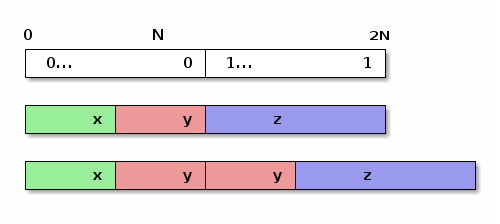
\includegraphics[width=.9\linewidth]{static/img/autospr/pumping_lema.png}
\end{center}

\subsection*{NEA (Nicht deterministische endliche Automaten}
\label{sec:org2929354}
NEAs unterscheiden sich von \hyperref[sec:org3b4cb19]{DEAs} nur geringfügig. Bei einem NEA ist es nicht notwendig, für jedes Zeichen einen Übergang zu haben. Zusätzlich können für das selbe Zeichen auch mehrere Übergänge existieren. Neben den bekannten Übergängen existieren im NEA auch \(\epsilon\)-Übergänge. Diese Übergänge können zu jeder Zeit, ohne ein Inputzeichen zu verwenden, benutzt werden.

NEAs können aber nicht mehr Sprachen erkennen als die DEAs. Sie sind daher gleichwertig.

Als Beispiel einen NEA, welcher Wörter erkennt, welche mit 2 b enden.
\begin{center}
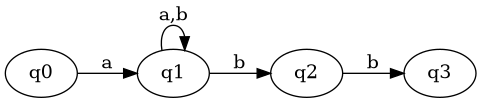
\includegraphics[width=.9\linewidth]{static/img/autospr/nea_example.png}
\end{center}

\subsection*{Thompson-NEA (Könnte-Automat)}
\label{sec:org0196cf4}
Bei diesem NEA wird sich immer gemerkt, in welchem Zustand der Automat sein könnte.

\subsection*{Transformation von NEA zu DEA}
\label{sec:orgb83404d}
Bei der Transformaiton von einem NEA zu einem DEA geht es darum, die \(\epsilon\)-Übergänge und die Mehrfachübergänge zu eliminieren. Das erreicht man, in dem der DEA Buch führt, in welchen Zuständen der NEA sein könnte. Das wird realisiert, in dem die Zustände des DEA die möglichen Zuständen des NEAs repräsentieren. Die Zustände \(Q\) des DEA ist die Potzenmenge der Menge \(Q\) des NEAs.

\subsubsection*{Beispiel}
\label{sec:org40388df}
Folgender NEA soll in einen DEA überführt werden:
\begin{center}
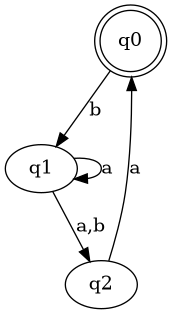
\includegraphics[width=.9\linewidth]{static/img/autospr/nea_example_2.png}
\end{center}

Dafür müssen die Potzenmenge der Zustände des NEAs gebildet werden:
\begin{itemize}
\item q\textsubscript{000} = \{\}
\item q\textsubscript{001} = \{q\textsubscript{0}\}
\item q\textsubscript{010} = \{q\textsubscript{1}\}
\item q\textsubscript{100} = \{q\textsubscript{2}\}
\item q\textsubscript{110} = \{q\textsubscript{2,q}\textsubscript{1}\}
\item q\textsubscript{101} = \{q\textsubscript{2,q}\textsubscript{0}\}
\item q\textsubscript{011} = \{q\textsubscript{1,q}\textsubscript{0}\}
\item q\textsubscript{111} = \{q\textsubscript{2,q}\textsubscript{1,q}\textsubscript{0}\}
\end{itemize}


Akzeptiertzustände sind alle welche den Status q\textsubscript{0} beinhalten => F = \{q\textsubscript{001}, q\textsubscript{101}, q\textsubscript{011}, q\textsubscript{111}\}. Startzustand ist q\textsubscript{001}. Nun kann das Zustandsdiagramm gezeichnet werden:  

\begin{center}
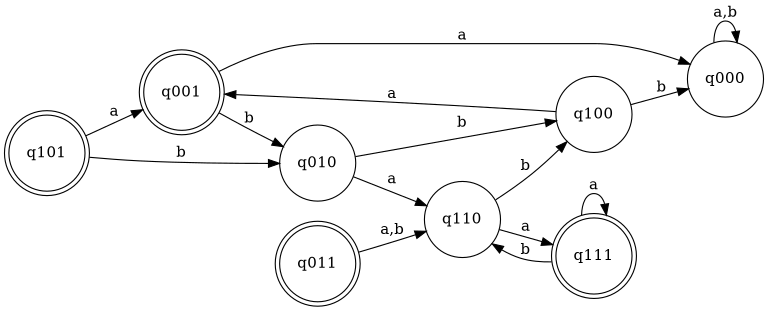
\includegraphics[width=.9\linewidth]{static/img/autospr/transformed_nea_example_2.png}
\end{center}

Im Bild ist ersichtlich, dass die Zustände q\textsubscript{101} und q\textsubscript{011} nie erreicht werden können und somit weggelassen werden können.

\subsection*{Mengenoperationen}
\label{sec:org143b963}
Sprachen sind Menge von Wörter. Folglich sind auch deren Vereinigung, Durchschnitt, Differenz etc. auch Sprachen. Wenn die Sprachen reguläre sind, ist auch dessen Vereinigung etc. Dies lässt sich mit einem NEA einfach beweisen.

\begin{figure}[htbp]
\centering
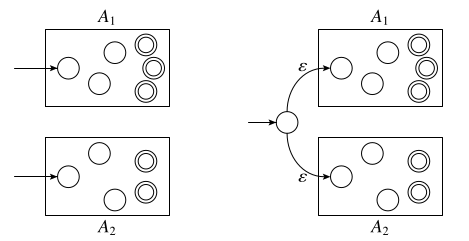
\includegraphics[width=.9\linewidth]{static/img/autospr/regulary_lang_cup.png}
\caption{Vereinigung zweicher Regulären Sprachen}
\end{figure}

Um die Schnittmenge zu bilden wird ein \textbf{kartesischer Produktautomat} benötigt.

\begin{center}
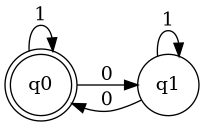
\includegraphics[width=.9\linewidth]{static/img/autospr/even_zero_dea.png}
\end{center}

\begin{center}
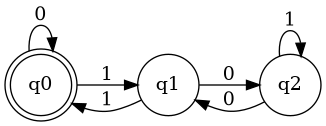
\includegraphics[width=.9\linewidth]{static/img/autospr/divide_by_3_dea.png}
\end{center}

\begin{figure}[htbp]
\centering
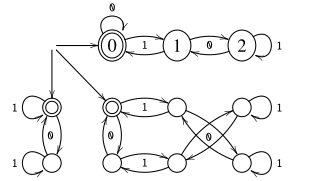
\includegraphics[width=.9\linewidth]{static/img/autospr/kartesischer_automata.png}
\caption{Kartesischer Produktautomat}
\end{figure}
\section*{Week 4}
\label{sec:orgc77991f}
\begin{itemize}
\item Reguläre Operationen
\begin{itemize}
\item Alternative
\item Verkettung
\item *-Operation
\end{itemize}
\item Umwandlung DEA <-> regulärer Ausdruck
\item Reguläre Ausdrücke in der Praxis
\begin{itemize}
\item Scanner-Generator flex
\item Performance von Regex-Engines
\end{itemize}
\end{itemize}


\subsection*{Reguläre Ausdrücke (Regex)}
\label{sec:org2dd8cf6}
Reguläre Ausdrücke sind eigentlich nichts anderes als eine kompakte Schreibweise für NEAs (folglich auch für DEAs).
\begin{center}
\begin{tabular}{ll}
Ausdruck & Bedeutung\\
\hline
a & das Zeichen \(a \in \Sigma\)\\
. & beliebiges Zeichen aus \(\Sigma\)\\
[aei] & ein Zeichen aus \({a, e, i} \subset \Sigma\)\\
[a-z] & für kleine Buchstaben von a-z\\
\(\epsilon\) & steht für das leere Wort\\
\(\emptyset\) & steht für die leere Sprach\\
\(r_{1}\vert r_{2}\) & Alternative\\
r* & Mehrfaches vorkommen von r\\
r+ & Mindestens einmal r\\
r? & 0 oder 1 mal r\\
\end{tabular}
\end{center}


\subsection*{DEAs in Regex umwandeln}
\label{sec:org34b96eb}
Jeder DEA kann mit Regex vereinfacht werden. Folgendes Vorgehen:
\begin{enumerate}
\item Neuer Akzeptiertzustand (q\textsubscript{accept}), alle andere werden zu normalen Zuständen degradiert und mit q\textsubscript{accept} verbunden
\item Neuer Startzustand (q\textsubscript{start}), andere werden zu normalen Zuständen degradiert und mit q\textsubscript{start} verbunden
\item Nach und nach alle Verbindungen raus nehmen und durch Regex reduzieren bis nur noch q\textsubscript{start} -> q\textsubscript{accept} vorig ist
\end{enumerate}

\section*{Week 5}
\label{sec:org7e1fd34}
\begin{itemize}
\item Kapitel 4: Stackautomaten und kontextfreie Sprachen
\begin{itemize}
\item Kontextfreie Grammatiken
\item Kontextfreie Sprachen
\item Beispiele
\item Reguläre Operationen für kontextfreie Grammatiken
\item Chomsky Normalform
\end{itemize}
\end{itemize}


\subsection*{Kontextfreie Sprachen}
\label{sec:org8a8ca94}
Eine kontextfreie Grammatik besteht aus:
\begin{itemize}
\item endliche Mengen von Variablen
\item endliche Menge von Zeichen (Terminalsymbole)
\item eine Menge von Regel
\item Eine Startvariabel
\end{itemize}


Kontextfrei bedeutet in diesem Fall, dass es auf der linken Seite der Regel immer nur eine Variabel gibt.
Kontextsensitive Regel:
$$
aA \rightarrow AA, bA \rightarrow BB
$$
Kontextfrei Regel:
$$
A \rightarrow AA
$$

Durch anwenden der Grammatik bis keine Variabel mehr übrigbleibt erzeugt eine \textbf{Kontextfreie Sprache}. Reguläre Sprachen sind eine Untermenge von kontextfreien Sprachen


\subsection*{Chomsky Normalform}
\label{sec:orge23ffb9}
Um zwei Grammatiken vergleichen zu können braucht es eine Normalform. Diese ist die Chomsky Normalform. Um in diese Form zu gelangen geht man wie folgt vor:
\begin{enumerate}
\item Die Startvariabel darf rechts nicht vorkommen. Notfalls eine neue Startvariabel S\textsubscript{0} erstellen mit der Regel \(S_0 \rightarrow S\)
\item Alle \(\epsilon\) Regel entfernen. Die einzige Ausnahme ist \(S_0 \rightarrow \epsilon\)
\item Entfernen von \emph{unit rules}: Regeln mit einer einzelnen Variabel auf der rechten Seite (\(A \rightarrow B\))
\item Verkettungen auflössen: \(A \rightarrow u_1A_1\). u\textsubscript{1} wird durch U\textsubscript{1} ersetzte und \(U_1 \rightarrow u_1\)
\end{enumerate}

\section*{Week 6}
\label{sec:org93b8bef}
\begin{itemize}
\item deterministischer Parse Algorithmus (Cocke-Younger-Kasami)
\item Stackautomaten
\begin{itemize}
\item Beispiel zur Motivation: \{0\textsuperscript{n1}\textsuperscript{n}| n ≥ 0\}
\item Formale Definition
\item Stackautomat als gerichterer beschrifteter Graph
\item Stackautomat einer kontextfreien Grammatik
\end{itemize}
\item Anwendung: Parser-Generator Bison
\end{itemize}


\subsection*{Cocke-Younger-Kasami}
\label{sec:org3147b06}
Um zu überprüfen, ob eine Wort zu einer kontextfreien Sprache gehört gibt es den \textbf{Cocke-Younger-Kasami}-Algorithmus. Dieser geht für das ganze Wort durch die Chomsky Normalform. Wenn es akzeptiert wird gehört es zu der Sprache ansonsten nicht.

\subsection*{Stackautomaten}
\label{sec:orgdb56d4c}
Stackautomaten sind DEAs welche mit einem Speicher, einem Stack, ausgestattet sind. So kann die 0 auf den Stack gespeichert werden bei der Sprache \({0^n1^n | n \in \mathbb{N}}\). Wenn der Stack am ende leer ist, wird das Wort akzeptiert. Bei Stackautomaten gibt es noch ein zusätzliches Alphabet, das Stack-Alphabet. Dieses wird verwendet um Symbole auf den Stack zu schreiben, bzw. von dort lesen.

Folgender Stackautomat, geht vom Zustand p nach q über, wenn ein a verarbeitet wird und gleichzeitig das Element c durch ein b ersetzt werden kann.
\begin{center}
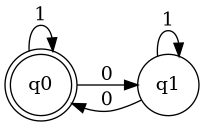
\includegraphics[width=.9\linewidth]{static/img/autospr/even_zero_dea.png}
\end{center}

\section*{Week 7}
\label{sec:org889e8fe}
\begin{itemize}
\item Pumping Lemma für kontextfreie Sprachen
\item Beispiel: \{ a\textsuperscript{n}b\textsuperscript{n}c\textsuperscript{n} | n \(\ge\) 0 \}
\item kontextfreie Grammatik eines Stackautomaten
\end{itemize}

\subsection*{Pumping Lemma für kontextfreie Sprachen}
\label{sec:orge3c4f3b}
Ähnliche wie bei Regulären Sprachen gibt es auch ein Pumping Lemma für kontextfreie Sprachen.

\begin{enumerate}
\item Annahme: L ist kontextfrei
\item Es gibt eine Pumping Length N
\item Wort: w = a\textsuperscript{N}b\textsuperscript{N}c\textsuperscript{N}
\item Wort in u, v, x, y, z zerlegen
\(|vy| > 0\), \(|vxy| \leq N\), \(uv^kxy^kz \in L \forall k \in \mathbb{N}\)
\item v und y aufpumpen
\item Widerspruch: L nicht kontextfrei
\end{enumerate}

\section*{Week 8}
\label{sec:org855c5c6}
\begin{itemize}
\item Kapitel 5: Turing Maschinen
\begin{itemize}
\item Definition Turing Maschine, erkannte Sprache
\item Zustandsdiagramm
\item Varianten (Bandalphabet, Anzahl Spuren, Anzahl Schreib-/Leseköpfe)
\item Aufzähler
\item Nicht deterministische Turingmaschinen
\end{itemize}
\end{itemize}

\begin{quote}
Jede nichtdeterministische Turingmaschine ist äquivalent zu einer deterministischen
Turingmaschine.
\end{quote}

\section*{Week 9}
\label{sec:org270d9f1}
\begin{itemize}
\item Abzählbar unendlich und überabzählbar unendlich
\item Die meisten Zahlen sind nicht berechenbar
\item Das 10. Hilbertsche Problem

\item Kapitel: 6 Entscheidbarkeit
\begin{itemize}
\item Akzeptanzprobleme für reguläre Sprachen
\item Leerheitsproblem für reguläre Sprachen
\item Gleichheitsproblem für reguläre Sprachen
\item Akzeptanzproblem für kontextfreie Sprachen
\item Leerheitsproblem für kontextfreie Sprachen
\item Gleichheitsproblem für kontextfreie Sprachen
\end{itemize}

\item Entscheidbarkeitsprobleme für kontextfreie Sprachen
\begin{itemize}
\item Akzeptanzproblem für kontextfreie Sprachen
\item Leerheitsproblem für kontextfreie Sprachen
\item Gleichheitsproblem für kontextfreie Sprachen
\end{itemize}

\item Halteproblem
\begin{itemize}
\item Akzeptanzproblem für Turing Maschinen Reduktion
\item Allgemeines Halteproblem
\item Leerheitsproblem für TM
\end{itemize}
\item Reduktion
\item Satz von Rice
\end{itemize}


\subsection*{Satz von Rice}
\label{sec:orgfa42e04}
\begin{quote}
Sei P eine nicht triviale Eigenschaft von Turing-erkennbaren Sprachen, dann
ist P nicht entscheidbar
\end{quote}
Nicht trivial meint, dass gewisse Sprachen die Eigenschaft haben und andere nicht.

\section*{Week 10}
\label{sec:org207de30}
\begin{itemize}
\item Kapitel 7: Komplexitätstheorie
\item Laufzeitkomplexität
\begin{itemize}
\item Definition der Laufzeit
\item Laufzeit für Varianten von Turingmaschinen
\end{itemize}

\item Komplexitätsklassen P und NP
\begin{itemize}
\item Beispiele von Sprachen in P
\item Verifizierer
\item Polynomielle Reduktion
\end{itemize}
\end{itemize}


\subsection*{Verifizierer}
\label{sec:orgbf5a5ef}
Wenn eine nichtdeterministische Turing Maschine ein Problem in polynomieller Zeit lösen kann, gibt es einen polynomieller Verifizieren. Ein polynomieller Verifizierer ist eine deterministische Turing Maschine, welche mit Hilfe eines Worts c (das Lösungszertifikat) überprüfen kann, ob das Wort w zu einer Sprache L gehört. Es gilt auch, wenn es einen Polynomieller Verifizierer gibt, dass eine nichtdeterministische TM in polynomieller Zeit entscheided.

Bsp: Eine nichtdetermistische Turing Maschine kann in polynomieller ein Sudoku lösen. Wenn man dem Verifiziere nun die Lösung des Sudokus gibt (die fehlenden Zahlen und deren Position), kann dieser in polynomieller Zeit die Lösung überprüfen / nachvollziehen.
\subsection*{Klasse P}
\label{sec:org627b27e}
\begin{quote}
Die Klasse P besteht aus den Sprachen, die mit einem Entscheider mit polyno-
mieller Laufzeit entschieden werden können.
\end{quote}

\subsection*{Klasse NP}
\label{sec:orgdcc0670}
\begin{quote}
Die Klasse der von einer nichtdeterministischen Turingmaschine in polynomi-
eller Zeit entscheidbaren Sprachen heisst NP.
\end{quote}
\subsection*{NP-Vollständig}
\label{sec:orgb0e0ffa}
NP-Vollständige Probleme sind die schwierigsten Probleme in NP. NP-Vollständige Probleme sind untereinander alle gleich schwierig zu lösen.
\begin{enumerate}
\item \(B \in NP\)
\item \(A \leq_p B \, \text{für alle} \, A \in NP\)
\end{enumerate}

\begin{center}
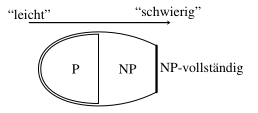
\includegraphics[width=.9\linewidth]{static/img/autospr/p_np_np_vollstaendig.png}
\end{center} 

\subsection*{Polynomielle Reduktion}
\label{sec:org9690234}
Die Polynomielle Reduktion ist die Idee, ein gegebenes Problem auf ein bekanntes Problem zu reduzieren.
Bsp: Stundenplan- und k-VERTEX-COLORING-Problem. Bei k-VERTEX-COLORING-Problem möchte man einen Graphen, mit k verschiedenen Farben so einfärben, dass kein Vertex die selbe Farbe hat, wie die Nachbarn. Die Reduktion vom Stundenplan auf k-VERTEX-COLORING sieht wie folgt aus:

\begin{itemize}
\item S -> k-VERTEX-COLORING
\item Fach -> Vertex
\item Zeitfenster -> Farbe
\item Anzahl Zeitfenster -> k
\item Student / Anmeldung -> Kante
\end{itemize}

Somit gilt: \$S \(\le\)\textsubscript{p} k-VERTEX-COLORING

\section*{Week 11}
\label{sec:org66b8c5f}
\begin{itemize}
\item SAT: Satz von Cook-Levin
\item Weitere Beispiele: 3SAT, k-CLIQUE, HAMPATH, SUBSET-SUM
\end{itemize}


\subsection*{Satz von Cook-Levin}
\label{sec:org75e306c}
\begin{quote}
SAT ist NP-vollständig.
\end{quote}

\section*{Week 12}
\label{sec:org74aa43f}
\begin{itemize}
\item Katalog von Karp
\item Minesweeper
\end{itemize}


\newpage
\subsection*{Katalog von Karp}
\label{sec:org45d7577}
\subsubsection*{SAT}
\label{sec:orgbb8004d}
\subsubsection*{CLIQUE}
\label{sec:org6638974}
\subsubsection*{VERTEX-COVER:}
\label{sec:org82cb532}
Gegeben ein Graph G und eine Zahl k, gibt es eine Teilmenge von k Vertizes so, dass jede Kante des Graphen ein Ende in dieser Teilmenge hat?

\subsubsection*{FEEDBACK-NODE-SET:}
\label{sec:orgb26e1c7}
Gegeben ein gerichteter Graph G und eine Zahl k, gibt es eine endliche Teilmenge von k Vertizes von G so, dass jeder Zyklus in G einen Vertex in der Teilmenge enthält?

\subsubsection*{FEEDBACK-ARC-SET:}
\label{sec:org2515ffa}
Gegeben ein gerichteter Graph G und eine Zahl k, gibt es eine Teilmenge von k Kanten so, dass jeder Zyklus in G eine Kante aus der Teilmenge enthält?

\subsubsection*{SET-COVERING:}
\label{sec:orgd6bea1c}
Gegeben eine endliche Familie endlicher Mengen (S j )1≤ j≤n und eine Zahl k, gibt es eine Unterfamilie bestehend aus k Mengen, die die gleiche Vereinigung hat?

\subsubsection*{EXACT-COVER:}
\label{sec:org2076a0a}
Gegeben eine Familie (S\textsubscript{j})\textsubscript{1 \(\le\) j \(\le\) n} von Teilmengen einer Menge U, gibt es eine Unterfamilie von Mengen, die disjunkt sind, aber die gleiche Vereinigung haben? Die Unterfamilie (S\textsubscript{ji})\textsubscript{1 \(\le\) i \(\le\) m} muss also S\textsubscript{ji} \(\cap\) S\textsubscript{jk} = \(\emptyset\) und
$$
\bigcup^n_{j=1} S_j = \bigcup^m_{i=1} S_{ji}
$$
erfüllen.

\section*{Week 13}
\label{sec:org7d1a823}
\begin{itemize}
\item Kapitel 8: Turing-Vollständigkeit

\begin{itemize}
\item Definition
\item Universelle Turing-Maschine
\item LOOP
\end{itemize}
\end{itemize}



\section*{End}
\label{sec:org2b64b61}
\end{multicols}
\end{document}